\documentclass[usenames,dvipsnames]{beamer}
\usepackage[utf8]{inputenc}
\usepackage[T1]{fontenc}
\usepackage[french]{babel}
\usepackage{xcolor}
\usepackage{pifont}
\usepackage{float}
\usetheme{Singapore} %Boadilla | Bergen | Madrid | Antibes | Hannover | Singapore | Warsaw

\newcommand{\cmark}{\ding{51}}
\newcommand{\xmark}{\ding{55}}
%----------------------------------------------------------------------------------------
%   TITLE INFORMATION
%----------------------------------------------------------------------------------------
\title{Entrepôts de données pour \textit{Tam voyages}}
\subtitle{HMIN122M -- Entrepôts de Données et Big-Data}
\author{B. Rima \and J. Saba \and T. Shaqura \and J. Bourgin}
\institute[UM]{M1 Informatique AIGLE}
\date{\today}

\begin{document}
%----------------------------------------------------------------------------------------
%   TITLE FRAME
%----------------------------------------------------------------------------------------
\begin{frame}
\titlepage
\end{frame}
%----------------------------------------------------------------------------------------
%   OUTLINE
%----------------------------------------------------------------------------------------
\begin{frame}{Sommaire}
\tableofcontents
\end{frame}
%----------------------------------------------------------------------------------------
%   INTRODUCTION
%----------------------------------------------------------------------------------------
\section{Introduction}
\begin{frame}{Contexte du projet}{Introduction}
\end{frame}

\section{Modélisation}
\begin{frame}{Contexte du projet}{Introduction}
\end{frame}

\subsection{Les Actions de TAM}
\begin{frame}{Modélisation}{Les Actions du TAM}
\section{Choix des actions à modéliser}
\begin{enumerate}
  \item \textbf{voyages}
  \item ventes
  \item \textbf{maintenance}
  \item amendes
\end{enumerate}
\begin{itemize}
  \item[] \textbf{voyages:} modèle en étoile détaillé.
  \item[] \textbf{maintenance:} record transaction.
\end{itemize}
\end{frame}

\subsection{Voyage Data Mart}
\begin{frame}{Data Mart Voyages}
\begin{figure}[!ht]
  \centering
  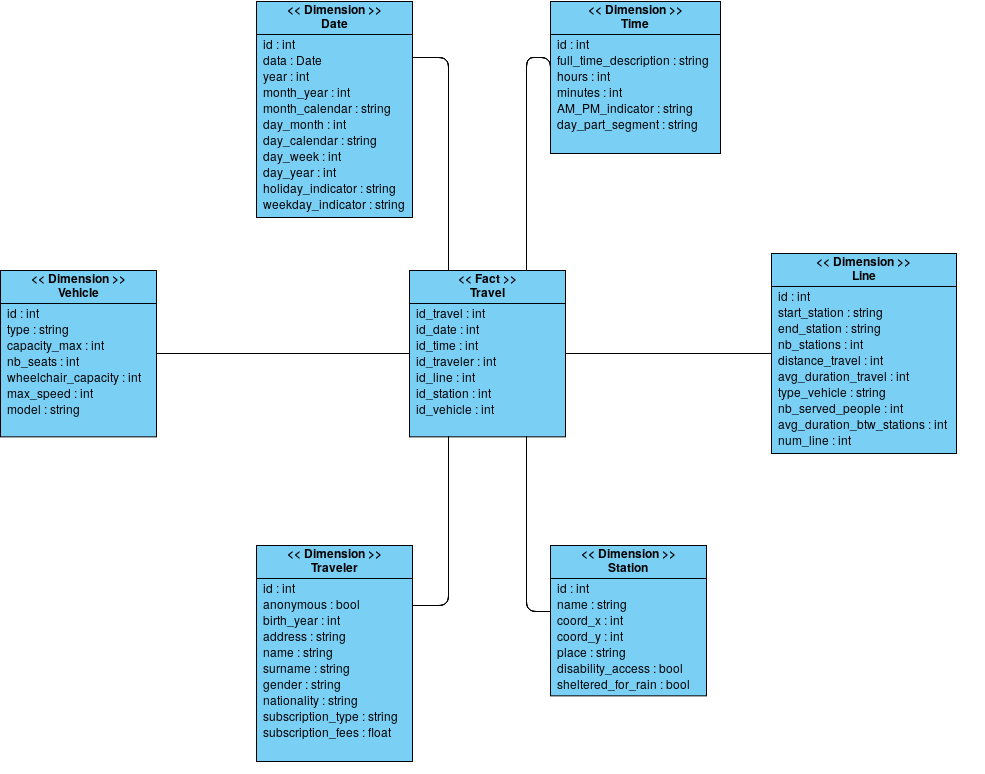
\includegraphics[width=0.9\textwidth]{images/voyages_datamart.png}
\end{figure}
\end{frame}

\subsection{Maintenance Data Mart}
\begin{frame}{Data Mart Maintenance}
\begin{figure}[!ht]
  \centering
  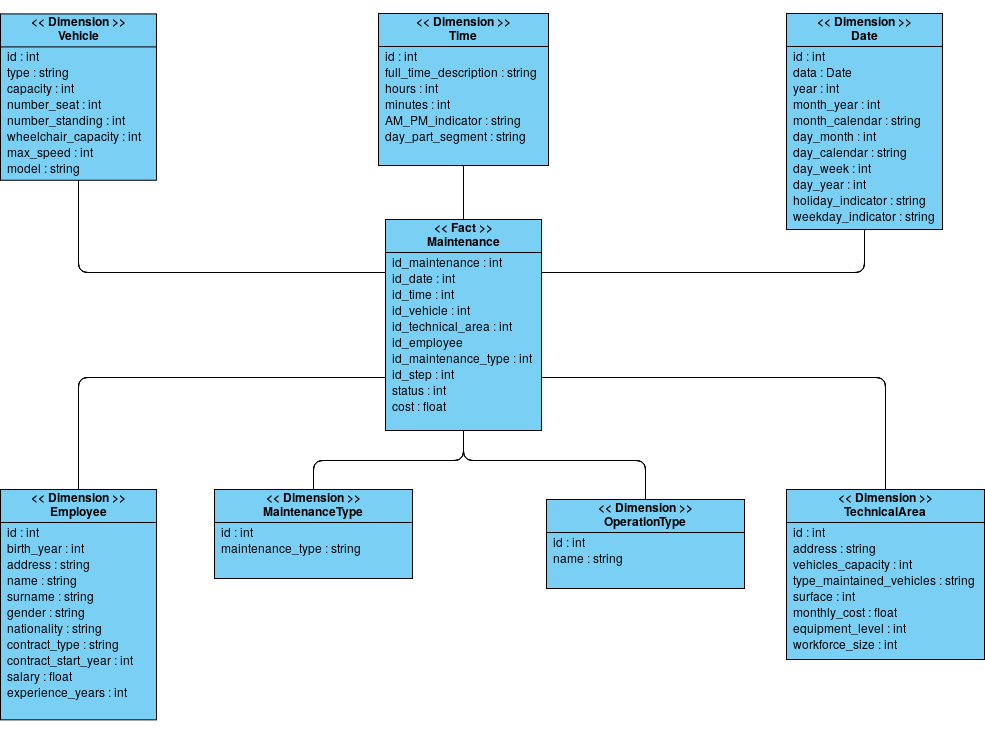
\includegraphics[width=0.9\textwidth]{images/maintenance_datamart.png}
\end{figure}
\end{frame}
\section{Implémentation}

\subsection{Data Warehouse}
\begin{frame}{Data Warehouse}
\begin{figure}[!ht]
  \centering
  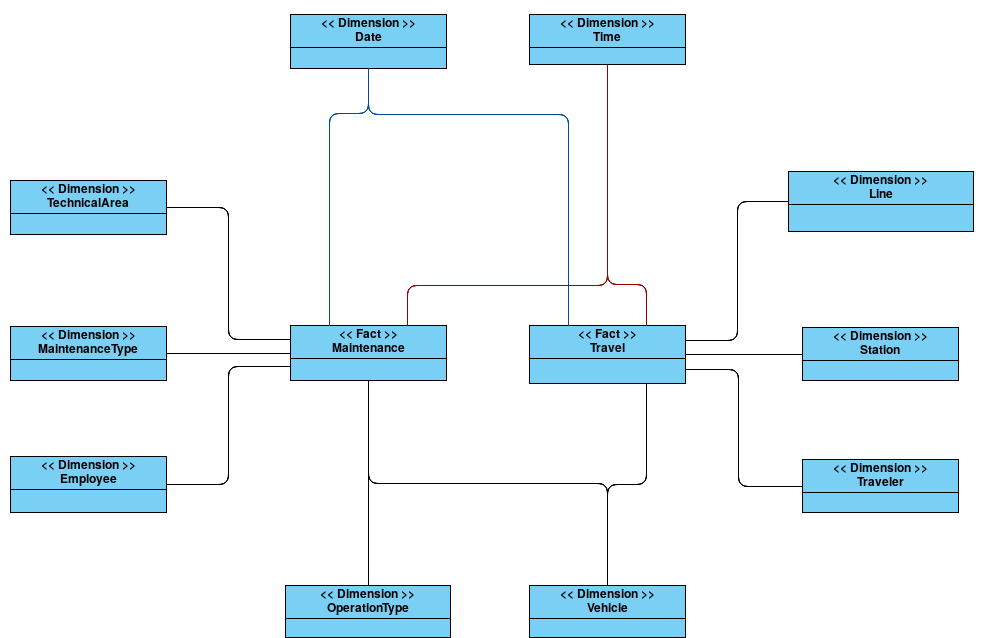
\includegraphics[width=0.9\textwidth]{images/data_warehouse.png}
\end{figure}
\end{frame}

\subsection{Estimation de la taille}
\begin{frame}{Estimation de la taille}
\begin{table}[!ht]
  \centering
  \begin{tabular}{|c|c|}
    \hline
    \textbf{Table} & \textbf{Taille}\\
    \hline
    \texttt{Date\_t} & $365$\\
    \hline
    \texttt{Time\_t} & $1440$\\
    \hline
    \texttt{Vehicle} & $270$\\
    \hline
    \texttt{Line} & $116$\\
    \hline
    \texttt{Station} & $654$\\
    \hline
    \texttt{TechnicalArea} & $2$\\
    \hline
    \texttt{MaintenanceType} & $\sim500$\\
    \hline
    \texttt{Employee} & $1144$\\
    \hline
    \texttt{Travel} & $128480000$\\
    \hline
  \end{tabular}
  \caption{taille estimée de chaque table de l'entrepôt}
\end{table}
\end{frame}

\begin{frame}{Contexte du projet}{Introduction}
\end{frame}

\section{Conclusion}
\begin{frame}{Contexte du projet}{Introduction}
\end{frame}
\end{document}
